\begin{figure}[ht]
    \centering
    % First bar plot (Pass@1 by Evaluation Steps)
    \begin{adjustbox}{minipage=\linewidth,scale=0.85}
        \begin{tikzpicture}
        \begin{axis}[
            width=0.32\linewidth,
            height=0.4\textheight,
            ybar,
            ylabel={Pass@1},
            symbolic x coords={Evaluation, Inference, Model Construction, Pre-Post Processing, Training},
            xtick=data,
            xticklabel style={rotate=90, anchor=east},
            bar width=15pt,
            nodes near coords,
            title={Pass@1 by Evaluation Steps},
            ymin=0, ymax=0.6,
            major grid style={dashed},
            grid=major,
            legend pos=north west
        ]
        \addplot coordinates {(Evaluation, 0.33) (Inference, 0.34) (Model Construction, 0.26) (Pre-Post Processing, 0.40) (Training, 0.35)};
        \draw[dashed, red] ({rel axis cs:0,0.34}) -- ({rel axis cs:1,0.34}) node[pos=1,above right] {0.34};
        \end{axis}
        \end{tikzpicture}
    \end{adjustbox}
    
    \hfill
    
    % Second bar plot (Pass@1 by Data Types)
    \begin{adjustbox}{minipage=\linewidth,scale=0.85}
        \begin{tikzpicture}
        \begin{axis}[
            width=0.32\linewidth,
            height=0.4\textheight,
            ybar,
            symbolic x coords={Image, Text, Tabled or Structured Array},
            xtick=data,
            xticklabel style={rotate=90, anchor=east},
            bar width=15pt,
            nodes near coords,
            title={Pass@1 by Data Types},
            ymin=0, ymax=0.6,
            major grid style={dashed},
            grid=major,
            legend pos=north west
        ]
        \addplot coordinates {(Image, 0.32) (Text, 0.32) (Tabled or Structured Array, 0.33)};
        \draw[dashed, red] ({rel axis cs:0,0.34}) -- ({rel axis cs:1,0.34}) node[pos=1,above right] {0.34};
        \end{axis}
        \end{tikzpicture}
    \end{adjustbox}
    
    \hfill
    
    % Third bar plot (Pass@1 by Task Types)
    \begin{adjustbox}{minipage=\linewidth,scale=0.85}
        \begin{tikzpicture}
        \begin{axis}[
            width=0.32\linewidth,
            height=0.4\textheight,
            ybar,
            symbolic x coords={Classification, Regression, Recommendation, Prediction, Detection, Segmentation},
            xtick=data,
            xticklabel style={rotate=90, anchor=east},
            bar width=15pt,
            nodes near coords,
            title={Pass@1 by Task Types},
            ymin=0, ymax=0.6,
            major grid style={dashed},
            grid=major,
            legend pos=north west
        ]
        \addplot coordinates {(Classification, 0.31) (Regression, 0.35) (Recommendation, 0.52) (Prediction, 0.32) (Detection, 0.22) (Segmentation, 0.30)};
        \draw[dashed, red] ({rel axis cs:0,0.34}) -- ({rel axis cs:1,0.34}) node[pos=1,above right] {0.34};
        \end{axis}
        \end{tikzpicture}
    \end{adjustbox}
    \label{fig:bar}
    \vspace{-10pt}

\end{figure}